% ------------------------------------------------------------------------------ %
% Pablo Rodríguez Guillén's personal template for all documents (at the moment)
% ------------------------------------------------------------------------------ %

\documentclass[11pt,a4paper]{article}

\usepackage[utf8]{inputenc}
\usepackage[spanish]{babel}
\usepackage[left=2.5cm,right=2.5cm,top=2.5cm,bottom=2.5cm]{geometry}

\usepackage[colorlinks = true, linkcolor = blue]{hyperref}
\usepackage{graphicx}
\usepackage{subfig}
\usepackage{listings}
\usepackage{url}

\author{Pablo Rodríguez Guillén \\ Profesor: Enrique García Salcines}
\title{\textbf{Fichero Aclaratorio Práctica 4: Expresiones regulares en Bash}}
\date{26 de mayo de 2019}

\setlength \parindent{0em}
\setlength \parskip{1em}

\begin{document}

% Uncomment for setting Bibliography without having to cite
% \nocite{*}

\maketitle
\tableofcontents
\newpage

\section{ejercicio1.sh}
El ejercicio hace uso principalmente del comando \emph{grep} con algunas de sus opciones, principalmente la opción \emph{--colour} que hace que el patrón que coincida con la expresión regular se resalte con color en la salida de pantalla. El comando \emph{sed} también es utilizado en el último apartado del ejercicio. A la salida de este se le aplica un grep para resaltar las modificaciones.

Cada uno de los apartados está codificado en el fichero \emph{ejercicio1.sh} y la explicación concreta de cada uno está disponible a través de comentarios de bash. Al inicio del script se encuentra la comprobación de errores al pasar el argumento, que debe ser un fichero. A continuación se muestra la primera parte de la ejecución del script, no se mostrará entera ya que la salida es extensa.

\begin{figure}[ht]
	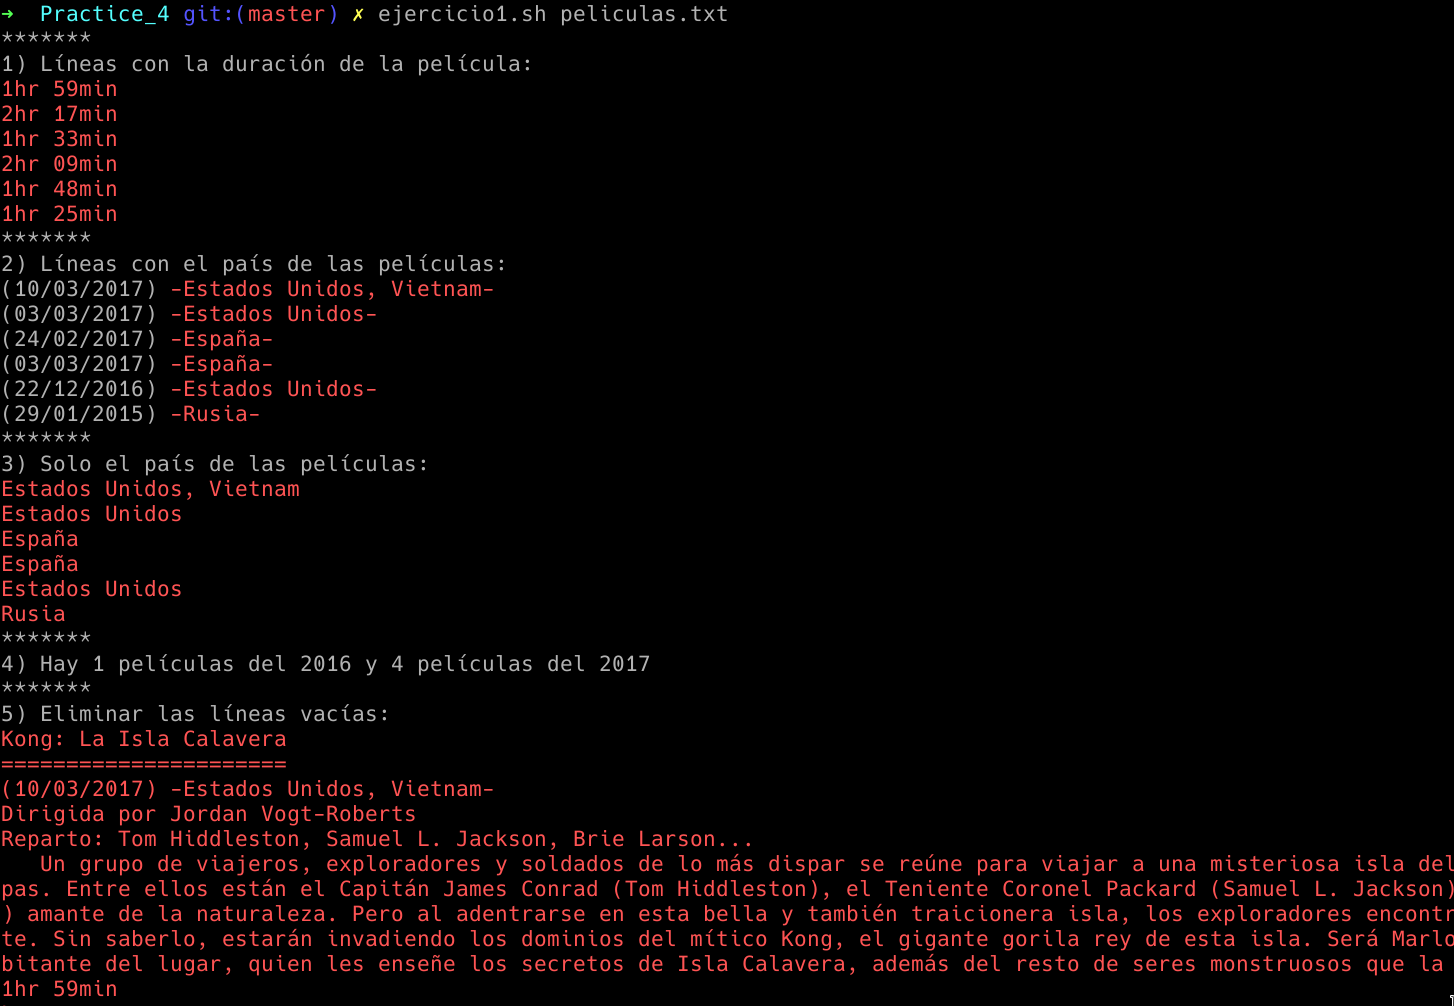
\includegraphics[width=1\textwidth]{images/ejercicio1.png}
	\caption{Salida de los 4 primeros apartados del ejercicio 1}
\end{figure}

\section{ejercicio2.sh}


% Uncomment for setting bibliography
% \addcontentsline{toc}{section}{Referencias}
% \bibliography{bibliography}
% \bibliographystyle{unsrt}

\end{document}
